% Figure: GTVH Analyzer, method overview.
% Compile:  pdflatex pipeline.tex   (produces pipeline.pdf, a cropped vector figure)
% Include:  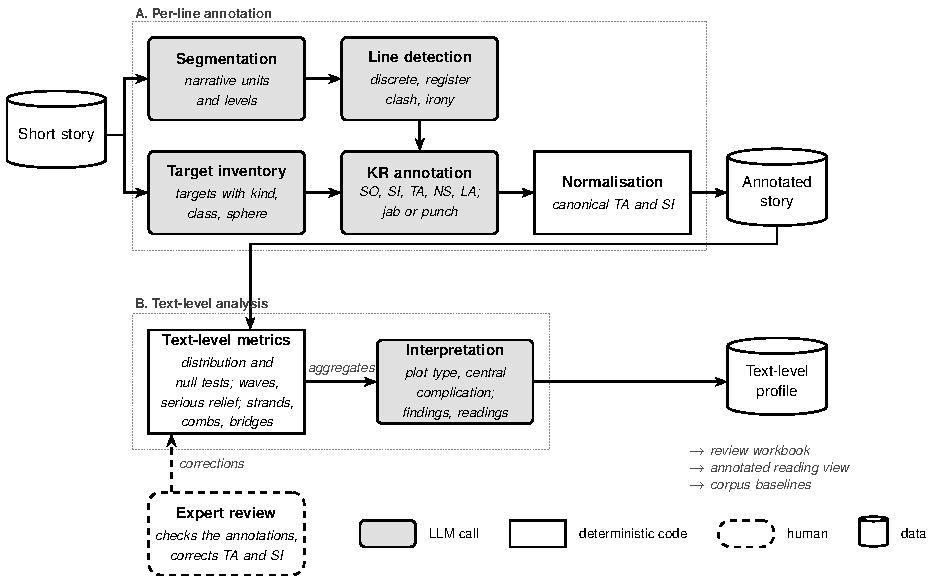
\includegraphics[width=\textwidth]{pipeline}
% Greyscale-safe: step types differ in fill, corners and line style, not colour.
% Natural width is about 15.5 cm, so it can be placed at full text width
% without shrinking the type.
\documentclass[border=3pt]{standalone}
\usepackage[T1]{fontenc}
\usepackage[scaled=0.92]{helvet}
\renewcommand{\familydefault}{\sfdefault}
\usepackage{tikz}
\usetikzlibrary{positioning, fit, arrows.meta, calc, shapes.geometric, backgrounds}

% No hyphenation inside the narrow boxes.
\hyphenpenalty=10000 \exhyphenpenalty=10000
\begin{document}
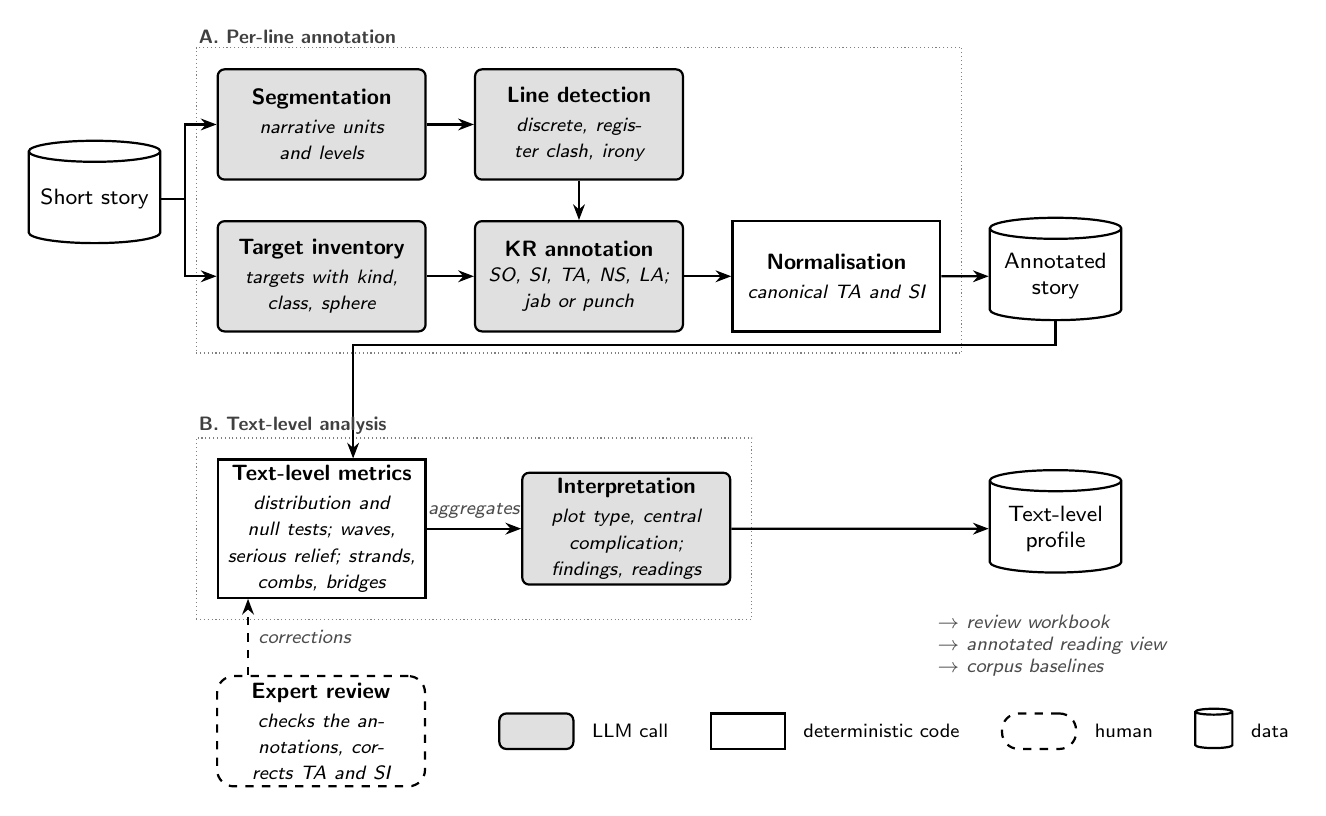
\begin{tikzpicture}[
  font=\footnotesize,
  node distance=4mm and 6mm,
  >={Stealth[length=2mm]},
  box/.style={thick, align=center, text width=25mm, minimum height=14mm, inner sep=2pt},
  llm/.style={box, draw, rounded corners=2.5pt, fill=black!12},
  code/.style={box, draw},
  human/.style={box, draw, dashed, rounded corners=6pt},
  data/.style={draw, thick, cylinder, shape border rotate=90, aspect=0.16, align=center,
               text width=16mm, minimum height=13mm, inner sep=1pt, fill=white},
  sub/.style={font=\scriptsize\itshape},
  note/.style={font=\scriptsize\itshape, text=black!70},
  phase/.style={draw=black!50, densely dotted, inner sep=2.6mm},
  phaselabel/.style={font=\scriptsize\bfseries, text=black!75, anchor=south west, inner sep=1pt},
  flow/.style={->, thick},
]

% ================= Row A: per-line annotation =================
\node[data] (story) {Short story};

\node[llm, right=7mm of story, yshift=9.5mm] (seg)
  {\textbf{Segmentation}\\[1pt]\scriptsize\itshape narrative units and levels};
\node[llm, below=5mm of seg] (inv)
  {\textbf{Target inventory}\\[1pt]\scriptsize\itshape targets with kind, class, sphere};

\node[llm, right=of seg] (det)
  {\textbf{Line detection}\\[1pt]\scriptsize\itshape discrete, register clash, irony};
\node[llm, below=5mm of det] (ann)
  {\textbf{KR annotation}\\[1pt]\scriptsize\itshape SO, SI, TA, NS, LA;\\ jab or punch};
\node[code, right=of ann] (norm)
  {\textbf{Normalisation}\\[1pt]\scriptsize\itshape canonical TA and SI};
\node[data, right=of norm] (corpus) {Annotated\\story};

\draw[flow] (story.east) -- ++(3mm,0) |- (seg.west);
\draw[flow] (story.east) -- ++(3mm,0) |- (inv.west);
\draw[flow] (seg) -- (det);
\draw[flow] (det) -- (ann);
\draw[flow] (inv) -- (ann);
\draw[flow] (ann) -- (norm);
\draw[flow] (norm) -- (corpus);

\begin{scope}[on background layer]
  \node[phase, fit=(seg)(inv)(det)(ann)(norm)] (A) {};
\end{scope}
\node[phaselabel] at (A.north west) {A. Per-line annotation};

% ================= Row B: review and text-level analysis =================
\node[code, below=16mm of inv.south west, anchor=north west] (metrics)
  {\textbf{Text-level metrics}\\[1pt]\scriptsize\itshape distribution and null tests; waves, serious relief; strands, combs, bridges};
\node[llm, right=12mm of metrics] (interp)
  {\textbf{Interpretation}\\[1pt]\scriptsize\itshape plot type, central complication; findings, readings};
\node[data] (profile) at (corpus |- interp) {Text-level\\profile};

\draw[flow] (metrics) -- node[note, above, pos=0.5] {aggregates} (interp);
\draw[flow] (interp) -- (profile);

% annotated story feeds the metrics
\draw[flow] (corpus.south) -- ++(0,-3mm) -| ($(metrics.north)+(4mm,0)$);

\begin{scope}[on background layer]
  \node[phase, fit=(metrics)(interp)] (B) {};
\end{scope}
\node[phaselabel] at (B.north west) {B. Text-level analysis};

% expert review: reads the annotated story, corrects canonical values
\node[human, below=7mm of B.south west, anchor=north west, xshift=2.6mm] (review)
  {\textbf{Expert review}\\[1pt]\scriptsize\itshape checks the annotations, corrects TA and SI};
\draw[flow, dashed] (review.north -| metrics.west) ++(4mm,0) coordinate (r)
      (review.north -| r) -- node[note, right, pos=0.5] {corrections} (metrics.south -| r);

% outputs of the whole pipeline, for readers
\node[note, align=left, anchor=north, text width=30mm] (outs) at ($(profile.south)+(0,-4mm)$)
  {$\rightarrow$ review workbook\\$\rightarrow$ annotated reading view\\$\rightarrow$ corpus baselines};

% ================= legend =================
\node[llm, text width=8mm, minimum height=4.5mm] (k1) at ($(review.east)+(14mm,0)$) {};
\node[right=1mm of k1, font=\scriptsize] (t1) {LLM call};
\node[code, text width=8mm, minimum height=4.5mm, right=4mm of t1] (k2) {};
\node[right=1mm of k2, font=\scriptsize] (t2) {deterministic code};
\node[human, text width=8mm, minimum height=4.5mm, right=4mm of t2] (k3) {};
\node[right=1mm of k3, font=\scriptsize] (t3) {human};
\node[data, text width=4mm, minimum height=5mm, right=4mm of t3] (k4) {};
\node[right=1mm of k4, font=\scriptsize] (t4) {data};

\end{tikzpicture}
\end{document}
